% ============================================================
%  Opportunistic Multimodal Constraint Satisfaction for
%  Robust Touchscreen Input Disambiguation
%  Self-contained academic paper
% ============================================================

\documentclass[11pt,letterpaper]{article}

\usepackage[T1]{fontenc}
\usepackage[utf8]{inputenc}
\usepackage[margin=1.1in,top=1.2in,bottom=1.2in]{geometry}
\usepackage{setspace}
\usepackage{titlesec}
\usepackage{enumitem}
\usepackage{amsmath}
\usepackage{amssymb}
\usepackage{parskip}
\usepackage{booktabs}
\usepackage{array}
\usepackage{xcolor}
\usepackage{hyperref}
\usepackage{cleveref}
\usepackage{float}
\usepackage{caption}
\usepackage{abstract}
\usepackage{tikz}
\usetikzlibrary{shapes.geometric, arrows.meta, positioning, fit, backgrounds}
\usepackage{fancyhdr}
\setlength{\headheight}{14.5pt}

% ---- Hyperref -----------------------------------------------
\hypersetup{
  colorlinks=true,
  linkcolor=black,
  urlcolor=black,
  citecolor=black,
  pdftitle={Opportunistic Multimodal Constraint Satisfaction for Robust Touchscreen Input},
  pdfauthor={Flyxion},
}

% ---- Typography ---------------------------------------------
\setstretch{1.18}
\setlength{\parindent}{0pt}
\setlength{\parskip}{7pt}

% ---- Section formatting -------------------------------------
\titleformat{\section}
  {\normalfont\large\bfseries}{\thesection.}{0.6em}{}
\titleformat{\subsection}
  {\normalfont\normalsize\bfseries}{\thesubsection.}{0.5em}{}
\titleformat{\subsubsection}[runin]
  {\normalfont\normalsize\itshape}{\thesubsubsection.}{0.4em}{}[.\quad]

% ---- Header / Footer ----------------------------------------
\pagestyle{fancy}
\fancyhf{}
\fancyhead[L]{\small\itshape Opportunistic Multimodal Constraint Satisfaction}
\fancyhead[R]{\small\itshape Flyxion}
\fancyfoot[C]{\thepage}
\renewcommand{\headrulewidth}{0.4pt}

% ---- Abstract box -------------------------------------------
\setlength{\absleftindent}{0.5cm}
\setlength{\absrightindent}{0.5cm}

% ============================================================
\begin{document}
% ============================================================

% ---- Title block --------------------------------------------
\begin{center}
  {\LARGE\bfseries Opportunistic Multimodal Constraint Satisfaction\\
  for Robust Touchscreen Input Disambiguation}\\[14pt]
  {\large Flyxion}\\[4pt]
  {\normalsize Independent Researcher, Canada}\\[4pt]
  {\normalsize\ttfamily github.com/standardgalactic}\\[10pt]
  {\normalsize\itshape Preprint --- \today}
\end{center}

\vspace{16pt}

% ---- Abstract -----------------------------------------------
\begin{abstract}
Capacitive touchscreens infer user intent from perturbations of an electrostatic
field. This single-modality architecture is fundamentally underdetermined: a
raindrop, a vibration artefact, and a deliberate fingertip contact can produce
indistinguishable local signatures. We propose a system that resolves this
underdetermination through opportunistic cross-modal constraint satisfaction. Under
normal conditions the system operates identically to a conventional touchscreen,
with no additional overhead or hardware dependency. When primary-signal confidence
falls below a dynamically adapted threshold---due to rain, mechanical vibration, or
weak-signal contact such as gloved operation---a secondary non-recording wearable
device is activated. This device, exemplified as lightweight glasses equipped with
optical or infrared sensing, provides real-time hand-motion and postural-context
data that is used to validate or reject candidate touch events. The wearable device
is defined by principled architectural incapacity: it cannot store imagery, transmit
raw sensor data, or produce a visual display, and these constraints are enforced in
hardware rather than software. The system additionally supports haptic glove input
as a screen-free channel, gated on a postural-context assessment that prevents
spurious input when the user's hands are not in a favourable configuration. We
describe the system architecture, the formal admissibility model, the operational
modes, and the relationship of the approach to prior work in gesture recognition,
sensor fusion, and gesture-based text entry. The design is offered as a defensive
public disclosure, placing the described methods in the public domain.

\smallskip\noindent\textbf{Keywords:} touchscreen disambiguation, multimodal input,
wearable sensing, constraint satisfaction, rain rejection, haptic input, defensive
publication.
\end{abstract}

\newpage

% ============================================================
\section{Introduction}
% ============================================================

The capacitive touchscreen has become the dominant human-computer interface modality
for portable devices. Its success rests on a simple and elegant physical principle:
a conducting finger perturbs an electrostatic field maintained across a sensing grid,
and the location and magnitude of that perturbation is decoded as a touch event.
Under controlled conditions this works well. Under real-world conditions it breaks
down in ways that have resisted satisfactory engineering solutions for over a decade.

The core difficulty is not one of signal fidelity but of \emph{underdetermination}.
From the perspective of the electrostatic grid, a raindrop impacting a glass surface
and a fingertip approaching deliberately are, in many configurations,
indistinguishable. Both are conducting stimuli of roughly the right size, arriving
at the surface with broadly similar temporal profiles. No amount of improvement to
the sensing grid itself can resolve this ambiguity, because the grid only has access
to the local surface perturbation. It has no view of what caused it.

Existing mitigations---spatial filtering, temporal thresholding, ``wet touch''
modes, oleophobic coatings, and perimeter moisture detectors---address symptoms
rather than causes. They tune the surface measurement to be less sensitive to certain
classes of false positive, at the cost of also being less sensitive to some true
positives. They cannot recover the missing information, because that information was
never available to the surface in the first place.

The solution we propose is to provide that missing information from an independent
source. A second sensing modality, geometrically distinct from the screen surface,
can observe the user's hand directly. It can answer questions that the surface
cannot: is a hand approaching at all? Is a finger extending toward the screen? Does
the timing and trajectory of that approach match the candidate touch event detected
at the surface? A raindrop cannot answer yes to these questions. A deliberate finger
contact typically can.

The challenge is to provide this second modality without introducing the privacy,
social, and architectural costs that have caused every previous attempt at
``smart glasses'' to fail or stall. We argue that this challenge is resolvable
through a principle we call \emph{principled incapacity}: the secondary device
is defined not only by what it does but by what it is architecturally prevented
from doing. A device that cannot record, cannot store, and cannot display is
qualitatively different from a general-purpose wearable computer. It occupies
the same social category as a keyboard or a mouse---a transient instrument
whose operation leaves no durable trace.

A second design principle is \emph{opportunistic activation}. The secondary device
is not always on. It is activated only when the primary signal falls below a
confidence threshold. Under normal dry conditions with steady hands, the system
is indistinguishable from a conventional touchscreen. The secondary device sits
idle, consuming negligible power, and imposes no latency. Only when conditions
degrade does it engage.

The result is a system that is robust where current systems are fragile, private
where smart glasses have been intrusive, and compatible with existing touchscreen
hardware without requiring any modification to the primary device.

The remainder of this paper is organised as follows. Section~\ref{sec:related}
surveys related work. Section~\ref{sec:model} presents the formal model.
Section~\ref{sec:architecture} describes the system architecture in detail.
Section~\ref{sec:modes} covers the operational modes. Section~\ref{sec:haptic}
addresses haptic glove integration. Section~\ref{sec:discussion} discusses the
broader significance of the approach, including its relationship to constraint-based
disambiguation in other domains. Section~\ref{sec:conclusion} concludes.

% ============================================================
\section{Related Work}
\label{sec:related}
% ============================================================

\subsection{Touchscreen Filtering and Environmental Compensation}

The most direct prior work is the body of engineering addressing adverse-condition
touchscreen performance. Manufacturers have introduced glove modes, which raise
sensitivity thresholds to respond to non-conductive or partially conductive contacts,
and wet-touch modes, which apply additional spatial and temporal filtering to suppress
the small, fast, scattered contacts characteristic of rain. Some devices include
capacitive moisture detectors at the screen perimeter that can trigger mode changes
when water is detected.

These approaches share a common limitation: they operate entirely within the local
surface measurement. Raising a sensitivity threshold helps with some false positives
but increases false negatives. Lowering it does the reverse. No threshold can
simultaneously improve both, because the signal distributions of intentional and
non-intentional contacts overlap. The problem is not filter design; it is the
absence of an independent discriminating signal.

\subsection{Optical and Depth-Based Gesture Recognition}

Gesture recognition systems using cameras, depth sensors, or time-of-flight
imaging have been extensively explored~\cite{gesture_survey}. These systems can
detect hand motion and infer gestures in free space with high accuracy. However,
they are almost universally designed as primary input modalities, replacing touch
rather than augmenting it. They depend on continuous scene capture, require
computational infrastructure for real-time scene understanding, and typically
produce persistent video or depth streams.

The present work differs in treating optical sensing as a secondary constraint
channel rather than a primary input channel. The wearable device does not need to
understand the scene; it only needs to answer a narrow set of questions about hand
position and motion. This dramatically reduces computational requirements and
eliminates the need for any persistent data capture.

\subsection{Smart Glasses and Augmented Reality}

Smart glasses platforms such as Google Glass, Microsoft HoloLens, and Meta Ray-Ban
demonstrate that wearable devices can provide useful spatial awareness. However, all
of these platforms include persistent recording capabilities, display surfaces, and
complex scene-understanding pipelines. The recording capability in particular has
generated substantial social resistance: bystanders cannot determine whether they
are being observed, and this ambiguity has limited adoption even in applications
where recording would be benign.

The device proposed here is distinguished from all of these by the principled
absence of recording and display. This is not a policy choice but a hardware
constraint, verifiable through attestation. The difference matters socially as much
as technically.

\subsection{Sensor Fusion in Mobile Devices}

Modern mobile devices fuse multiple co-located sensors---accelerometers, gyroscopes,
proximity sensors, barometers, and ambient light sensors---to improve orientation
estimation, context awareness, and power management. The fusion is entirely internal
to the device.

The present work extends sensor fusion across physically separate devices, adding an
external wearable viewpoint to the sensing ensemble. This is qualitatively different
from intra-device fusion: the wearable provides a perspective from which both the
user's hands and the screen surface are simultaneously observable, a viewpoint the
device itself cannot achieve.

\subsection{Gesture-Based Text Entry and Disambiguation}

The Swype keyboard~\cite{swype} offers an instructive structural parallel. Swype
accepts a continuous swipe trajectory across a touchscreen and maps it to a word by
projecting the trajectory into a constrained linguistic space: the user's lexicon,
weighted by frequency priors and personal usage history. The raw gesture is
underdetermined---many words correspond to any given trajectory---and the lexicon
provides the constraint that selects among them.

The present system performs an analogous disambiguation at a lower level of the
input stack. Rather than asking which symbol a trajectory encodes, it asks whether
a surface event encodes any deliberate act at all. The constraint is physical and
kinematic rather than linguistic, but the structural principle is identical: raw
input is not trusted in isolation and must be brought into agreement with an
independent constraint source before being admitted. We return to this analogy in
Section~\ref{sec:discussion}.

\subsection{Air Typing and Haptic Glove Input}

Air-typing and haptic-glove systems encode finger flexion and contact events as
symbolic input without requiring physical contact with a surface~\cite{airtype}.
These systems have demonstrated reasonable accuracy in controlled settings but
share a common weakness: they do not account for postural context. A virtual
keyboard projected in front of the user is not useful when the user's hands are
at their sides, when the user is walking, or when gaze is directed elsewhere.
Without postural gating, glove-mode input generates spurious events whenever
the user's hands move for non-input purposes.

The present work integrates haptic glove input within the same constraint framework
as touch disambiguation and explicitly gates glove-mode activation on a
postural-context assessment derived from the wearable device.

% ============================================================
\section{Formal Model}
\label{sec:model}
% ============================================================

\subsection{Primary Event Stream}

The primary input device produces a stream of candidate touch events:
\[
  \mathcal{E} = \bigl\{\, e_i = (x_i,\, y_i,\, t_i,\, s_i,\, \sigma_i) \bigr\}
\]
where $(x_i, y_i)$ are screen coordinates, $t_i$ is the detection timestamp,
$s_i$ is the integrated signal strength, and $\sigma_i \in [0,1]$ is a
per-event confidence score. The confidence score is produced by a local classifier
whose features include signal morphology, contact-area distribution, approach
velocity (where derivable from the temporal signal profile), and the current
estimated false-positive rate.

\subsection{Adaptive Threshold}

The confidence monitor maintains a sliding-window estimate of the ambient
false-positive rate $\hat{f}(t)$ and reads vibration magnitude $v(t)$ from the
device accelerometer. The acceptance threshold is:
\begin{equation}
  \tau(t) = \tau_0 + \alpha\,\hat{f}(t) + \beta\,v(t)
  \label{eq:threshold}
\end{equation}
where $\tau_0$ is a baseline threshold and $\alpha, \beta$ are tunable weights.
Under calm, dry conditions $\tau(t) \approx \tau_0$ and nearly all events satisfy
$\sigma_i \geq \tau(t)$, proceeding directly to the host application. Under rain
or vibration $\tau(t)$ rises, causing more events to be held pending cross-modal
validation.

\subsection{Constraint Signal}

When activated, the wearable device produces a constraint signal stream:
\[
  \mathcal{C} = \bigl\{\, c_j = (\mathbf{p}_j,\, \mathbf{v}_j,\, \phi_j,\,
  t_j,\, \psi_j) \bigr\}
\]
where $\mathbf{p}_j \in \mathbb{R}^3$ is the estimated fingertip position in a
shared coordinate frame, $\mathbf{v}_j$ is its velocity vector, $\phi_j \in [0,1]$
is finger-extension confidence, $t_j$ is the observation timestamp, and $\psi_j
\in \{0,1\}$ is a postural-context flag (defined in Section~\ref{sec:haptic}).

\subsection{Admissibility}

A held candidate event $e_i$ is admitted if and only if $A(e_i, \mathcal{C}) = 1$,
where admissibility is the conjunction of three conditions.

\paragraph{Temporal correlation.}
\[
  \exists\, c_j \in \mathcal{C} : |t_i - t_j| \leq \Delta t
\]
where $\Delta t$ is a configurable temporal window (default 120\,ms). This
condition eliminates environmental events that have no associated hand motion.

\paragraph{Spatial intersection.}
\[
  \bigl\| \pi(\mathbf{p}_j) - (x_i, y_i) \bigr\| \leq r
\]
where $\pi : \mathbb{R}^3 \to \mathbb{R}^2$ is the coordinate-frame registration
transform (Section~\ref{sec:calibration}) and $r$ is a tolerance radius (default
8\,mm). This condition requires that the observed hand position projects onto the
screen region of the candidate event.

\paragraph{Motor plausibility.}
The velocity profile $\mathbf{v}_j$ and the finger-extension sequence leading to
$c_j$ must be consistent with voluntary reach-and-contact motion. Criteria include:
approach velocity within a characteristic range $[v_{\min}, v_{\max}]$,
monotonically decreasing finger-to-screen distance over the preceding window, and
absence of lateral scatter inconsistent with directed motion.

Events satisfying all three conditions are promoted to the host application as
validated input. Events failing any condition are classified into one of three
rejection classes: \emph{environmental noise} (no temporally proximate constraint
observation, e.g.\ rain or condensation), \emph{vibrational artefact} (constraint
observation present but motor plausibility absent), or \emph{non-directed contact}
(hand present but approach not directed toward the event location).

% ============================================================
\section{System Architecture}
\label{sec:architecture}
% ============================================================

\subsection{Overview}

Figure~\ref{fig:arch} illustrates the high-level architecture. The primary input
device generates candidate events, which the confidence monitor evaluates against
the adaptive threshold $\tau(t)$. Events meeting the threshold are forwarded
directly to the host application. Events below threshold are held and routed to
the fusion module, which activates the wearable constraint device and evaluates
cross-modal admissibility.

% ---- Figure 1 -----------------------------------------------
\begin{figure}[H]
\centering
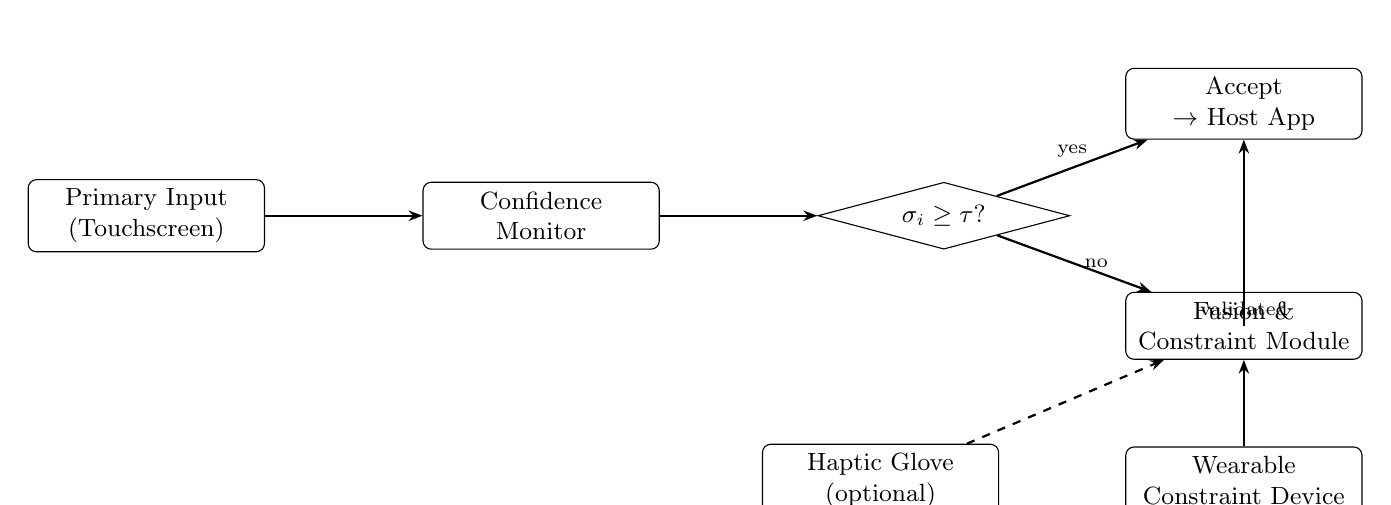
\begin{tikzpicture}[
  node distance = 1.3cm and 2.0cm,
  box/.style     = {rectangle, draw, rounded corners=3pt,
                    minimum width=3.0cm, minimum height=0.85cm,
                    font=\small, align=center},
  decision/.style= {diamond, draw, aspect=2.4,
                    minimum width=3.2cm, minimum height=0.85cm,
                    font=\small, align=center, inner sep=1pt},
  arr/.style     = {-{Stealth[length=5pt]}, thick},
  dasharr/.style = {-{Stealth[length=5pt]}, thick, dashed},
]
\node[box] (screen)   {Primary Input\\(Touchscreen)};
\node[box, right=of screen] (mon) {Confidence\\Monitor};
\node[decision, right=of mon] (dec) {$\sigma_i \geq \tau$?};
\node[box, above right=0.75cm and 1.5cm of dec] (ok)  {Accept\\$\to$ Host App};
\node[box, below right=0.75cm and 1.5cm of dec] (fus) {Fusion \&\\Constraint Module};
\node[box, below=1.1cm of fus] (gl)  {Wearable\\Constraint Device};
\node[box, left=1.6cm of gl]   (glv) {Haptic Glove\\(optional)};

\draw[arr]    (screen) -- (mon);
\draw[arr]    (mon)    -- (dec);
\draw[arr]    (dec)    -- node[above,font=\scriptsize]{yes} (ok);
\draw[arr]    (dec)    -- node[right,font=\scriptsize]{no}  (fus);
\draw[arr]    (gl)     -- (fus);
\draw[dasharr](glv)    -- (fus);
\draw[arr]    (fus)    -| node[above,font=\scriptsize,pos=0.28]{validated} (ok);
\end{tikzpicture}
\caption{System architecture. The wearable constraint device is activated only when
primary-signal confidence falls below the adaptive threshold $\tau(t)$. The haptic
glove channel (dashed) is additionally gated on postural context $\psi_j$.}
\label{fig:arch}
\end{figure}

\subsection{Primary Input Device}

The primary device requires no hardware modification beyond existing touchscreen
designs. It contributes the event stream $\mathcal{E}$, the confidence scores
$\sigma_i$, and the environmental readings (accelerometer, barometer, optional
moisture detector) used by the confidence monitor to compute $\tau(t)$.

\subsection{Wearable Constraint Device}

The preferred physical embodiment is lightweight glasses. Alternative embodiments
include a headband, an ear-mounted unit, or a shoulder-mounted sensor. The
requirement common to all embodiments is a viewpoint from which both the user's
hands and the device screen are simultaneously observable.

Sensing hardware comprises one or more of: a monocular or stereo RGB or monochrome
camera; an infrared illuminator with corresponding IR sensor for low-light operation;
a time-of-flight depth sensor; and an inertial measurement unit for head-pose
estimation. The device communicates with the host via a low-latency wireless
protocol (e.g.\ Bluetooth Low Energy with a custom constraint-data profile),
transmitting only the derived signal $\mathcal{C}$. Raw imagery is never transmitted.

The device is subject to the following hardware constraints, enforced through
physical design and verified by a secure-element attestation mechanism:

\begin{itemize}[leftmargin=2em, itemsep=2pt]
  \item No non-volatile storage. All sensor data is processed in working memory and
        discarded within a bounded window not exceeding 500 milliseconds.
  \item No display surface, projector, or optical combiner.
  \item The wireless interface is read-only with respect to raw sensor data; only
        derived constraint signals conforming to the specified protocol may be
        transmitted.
\end{itemize}

These constraints place the device in a qualitatively different category from
existing wearable computers. It behaves as a measuring instrument rather than a
recording device, analogous to a thermometer or a mouse: it produces a transient
output signal and retains no record of the environment.

\subsection{Coordinate Frame Registration}
\label{sec:calibration}

Cross-modal spatial correlation requires that the constraint signal $\mathbf{p}_j$
and the screen coordinates $(x_i, y_i)$ be expressed in a common frame. Registration
is performed at pairing time via a brief calibration procedure: the user touches a
sequence of prompted targets, and the fusion module records simultaneous screen and
wearable observations. A rigid-body projection $\pi : \mathbb{R}^3 \to \mathbb{R}^2$
is estimated by least-squares minimisation over the calibration pairs and updated
incrementally as validated events accumulate during normal use, accommodating
gradual drift from changes in wearable fit or device orientation.

\subsection{Fusion and Constraint Evaluation}

The fusion module maintains a short event buffer holding candidate events awaiting
cross-modal validation. When the wearable is active, each buffered event is evaluated
against the admissibility conditions of Section~\ref{sec:model}. Admitted events are
forwarded with a latency not exceeding $\Delta t + d_{\text{comm}}$, where
$d_{\text{comm}}$ is the wireless round-trip time (target: $\leq 30$\,ms), giving
a worst-case additional latency of approximately 150\,ms relative to a direct
touch event.

A per-session rejection log is maintained in volatile memory to support adaptive
threshold adjustment. This log is not persisted beyond the current session.

A personalised motor model $\mathcal{M}_u$ is maintained in local encrypted storage
on the host device and is updated as the user accumulates validated input events.
Over time this model refines the motor-plausibility classifier to the specific
approach velocities, angles, and inter-event timing of the individual user, reducing
false negatives without increasing false positives. The model is device-local and is
not transmitted to any external system.

% ============================================================
\section{Operational Modes}
\label{sec:modes}
% ============================================================

\subsection{Normal Mode}

The system operates as a conventional touchscreen. The wearable is in low-power
idle. All candidate events satisfy $\sigma_i \geq \tau(t)$ and are forwarded
directly to the host application. This is the predominant mode under dry, stable
conditions.

\subsection{Rain and Moisture Rejection Mode}

Activated when $\hat{f}(t)$ exceeds a moisture-onset threshold or when a perimeter
moisture detector reports wet conditions. The threshold $\tau(t)$ rises according
to~\eqref{eq:threshold}. The wearable is activated. Touch events require
cross-modal confirmation. Events lacking a temporally proximate constraint
observation are classified as environmental noise and discarded.

The user experience is transparent: deliberate touches continue to register while
raindrops are suppressed, at the cost of the validation latency for events that
require cross-modal confirmation. In practice, deliberate touches during rain tend
to be slower and more deliberate than normal, so the additional latency is largely
masked by the approach trajectory itself.

\subsection{Vibration Rejection Mode}

Activated when accelerometer RMS exceeds a vibration threshold, as occurs on
trains, aircraft, or during seismic events. The $\beta\,v(t)$ term in
\eqref{eq:threshold} raises the acceptance threshold. The motor-plausibility
condition is particularly effective in this mode: vibration-induced contact events
lack directed approach trajectories, while intentional touches during vibration
are characterised by a bracing-and-reaching motion profile that is detectably
different.

\subsection{Weak-Signal and Glove Mode}

Activated when $s_i$ falls below a glove-detection threshold, indicating a
non-conductive or partially conductive contact. The wearable becomes the primary
signal source, and contact is inferred from finger trajectory rather than surface
perturbation. The electrostatic grid continues to contribute coarse positional data
when available but is not required for event validation.

% ============================================================
\section{Haptic Glove Integration}
\label{sec:haptic}
% ============================================================

\subsection{Postural Context}

The postural-context flag $\psi_j$ encodes whether the user's current body
configuration is favourable for deliberate input. The wearable assesses three
conditions: (1) hand elevation consistent with active input rather than resting
or conversational gesture; (2) head orientation, estimated from the IMU, directed
toward the expected input region (a coarse estimate, not requiring eye tracking);
and (3) hand and head motion below a stability threshold. $\psi_j = 1$ when all
three conditions are met; $\psi_j = 0$ otherwise.

\subsection{Glove Input Channel}

Haptic gloves encode finger flexion, extension, and contact events as symbolic
input without requiring screen contact. Within the present framework, glove-generated
events are treated as candidate inputs subject to the same constraint evaluation
as touch events, with the addition that the entire glove channel is suspended when
$\psi_j = 0$.

This postural gating is the key distinction from prior air-typing systems. It
prevents spurious input events from being generated when the user's hands move for
non-input purposes: walking, talking with the hands, reaching for objects, or simply
resting. The channel activates automatically when the user adopts an input posture
and suspends automatically when they leave it, requiring no explicit mode switching
by the user.

\subsection{Virtual Layout Anchoring}

When $\psi_j = 1$, the fusion module anchors a virtual input layout---a keyboard
or gesture vocabulary---to the user's physical configuration as derived from the
wearable. Repeated finger-motion trajectories are clustered to identify stable
symbolic mappings. The layout adapts over time to the user's natural hand position
and reach geometry, converging toward a stable, personalised mapping rather than
requiring the user to conform to a fixed virtual layout.

% ============================================================
\section{Discussion}
\label{sec:discussion}
% ============================================================

\subsection{Constraint Satisfaction as a Unifying Principle}

The core contribution of this work is not a specific sensing technology but a
reframing of the touch-input problem. Current systems treat touch interpretation as
a \emph{classification problem within a single modality}: given the signal at the
surface, determine the most likely input event. We propose treating it as a
\emph{constraint satisfaction problem across modalities}: an input event is admitted
only when it satisfies constraints imposed independently by two or more sensing
channels.

This reframing has a well-known analogue in text entry. The Swype gesture keyboard
accepts an inherently ambiguous swipe trajectory and resolves it by projecting into
a constrained space defined by the user's lexicon. The raw signal is not trusted on
its own. It must agree with an independent constraint---language statistics and
personal vocabulary---before a specific symbol is committed.

The present system applies the same strategy at the level of physical intent rather
than symbolic identity. A touch event is not committed until it agrees with an
independent observation of hand motion. The constraint is kinematic and spatial
rather than lexical, but the structural principle is identical: raw recurrence
(repeated surface perturbations) is resolved by cross-channel constraint into
stable output (validated intentional input).

This principle generalises beyond the specific embodiments described here. Any
situation in which a primary signal is underdetermined can potentially be stabilised
by coupling it to an independent constraint channel, provided that the sources of
noise in the primary channel are unlikely to simultaneously satisfy the constraint.
Rain satisfies neither temporal correlation with directed hand motion nor motor
plausibility. Vibration artefacts satisfy temporal correlation but not motor
plausibility. Palm contact satisfies spatial proximity but not directed approach.
Each noise source fails at a different point in the admissibility chain.

\subsection{Why Previous Smart Glasses Approaches Failed}

The history of consumer smart glasses has been one of technically capable devices
that failed for social and architectural reasons rather than sensing limitations.
The primary issues have been the recording capability and the display: bystanders
cannot determine what the device is capturing, and the display creates a visible
barrier between the wearer and their social environment.

The device proposed here is architected to avoid both issues by exclusion rather
than policy. There is nothing to record because there is no storage. There is
nothing to display because there is no display surface. The hardware attestation
mechanism makes these absences verifiable rather than merely asserted. A device
whose incapacities are demonstrable occupies a different social and regulatory
category from one that merely promises not to use capabilities it possesses.

The device is, in this respect, more analogous to a barcode scanner or a motion
sensor than to a camera. Its outputs are narrow, structured, and transient. It has
no general-purpose sensing capability that could be redirected toward surveillance.
This narrowness is a feature rather than a limitation.

\subsection{Graceful Degradation}

A design requirement not always emphasised in multimodal systems is graceful
degradation: the system should not perform worse when auxiliary devices are absent
than a conventional system without them. The present design satisfies this
requirement by construction. When the wearable is unavailable, the system reverts
to conventional single-surface inference. When the wearable is idle, it imposes
no latency or power overhead. The auxiliary channel is strictly additive.

\subsection{Privacy}

The system transmits no biometric data in the conventional sense: no face images,
no gaze direction, no voice. The constraint signal encodes only coarse hand position
and velocity, which are not individually identifying. The personalised motor model
is stored locally and not transmitted. The system does not require network
connectivity to function.

\subsection{Limitations and Future Work}

The primary limitation of the current design is the calibration requirement. The
coordinate-frame registration between the wearable and the screen requires an
explicit calibration step at pairing time and periodic re-calibration as device
position or wearable fit changes. Future work could address this through continuous
self-calibration using validated touch events as ground truth, reducing or
eliminating the explicit calibration step.

A second limitation is the validation latency. The worst-case additional latency
of approximately 150\,ms is imperceptible for many interactions but may be
noticeable for rapid tap sequences. Future work could reduce this by predictive
pre-activation of the wearable when environmental conditions suggest imminent
degradation, reducing the latency of the first event in a degraded-condition
sequence.

The motor-plausibility classifier described here is relatively simple. Richer
models trained on larger datasets of intentional versus non-intentional contacts
across a range of environmental conditions would improve accuracy, particularly
in novel adverse conditions not well represented in the training data.

% ============================================================
\section{Conclusion}
\label{sec:conclusion}
% ============================================================

We have described a system for robust touchscreen input disambiguation based on
opportunistic cross-modal constraint satisfaction. The system introduces a secondary
non-recording wearable device that provides real-time hand-motion constraint data,
activated only when primary-signal confidence is insufficient. Input events are
admitted only when they satisfy temporal, spatial, and motor-plausibility conditions
across both sensing modalities simultaneously. The wearable device is defined by
principled architectural incapacity---it cannot record, store, or display---placing
it in a social and regulatory category distinct from existing smart glasses systems.
A haptic glove input channel is integrated within the same constraint framework,
gated on a postural-context assessment that prevents spurious input outside
deliberate input postures.

The approach reframes touch input from a single-modality classification problem to
a cross-modal constraint satisfaction problem, a reframing with structural analogues
in gesture-based text entry and other domains where raw signals are underdetermined
relative to intended outputs.

This paper is offered as a defensive public disclosure. The methods described are
hereby placed in the public domain. No patent protection is claimed, and the authors
encourage free implementation and extension of these ideas.

\newpage
% ============================================================
%  References
% ============================================================
\begin{thebibliography}{9}

\bibitem{gesture_survey}
Rautaray, S.~S. and Agrawal, A. (2015).
Vision based hand gesture recognition for human computer interaction: a survey.
\textit{Artificial Intelligence Review}, 43(1), 1--54.

\bibitem{swype}
Zhai, S. and Kristensson, P.-O. (2012).
The word-gesture keyboard: reimagining keyboard interaction.
\textit{Communications of the ACM}, 55(9), 91--101.

\bibitem{airtype}
Nirjon, S., Gummeson, J., Gelb, D., and Kim, K.-H. (2015).
Typingring: a wearable ring platform for text input.
\textit{Proceedings of MobiSys}, 155--166.

\bibitem{tof_hand}
Sridhar, S., Oulasvirta, A., and Theobalt, C. (2013).
Interactive markerless articulated hand motion tracking using RGB and depth data.
\textit{Proceedings of ICCV}, 2456--2463.

\bibitem{moisture}
Goel, M., Wobbrock, J., and Patel, S. (2012).
GripSense: using built-in sensors to detect hand posture and pressure on commodity
mobile phones.
\textit{Proceedings of UIST}, 545--554.

\end{thebibliography}

\vspace{16pt}
\hrule
\vspace{8pt}
\noindent\small\textit{This work is released as a defensive public disclosure.
The described methods are placed unconditionally in the public domain as of the
date of first publication. No patent application has been filed. The authors assert
no proprietary rights over the techniques described herein and encourage free
use, implementation, and extension.}

\end{document}